\documentclass{ximera}
\graphicspath{
{./}
{volumes/}
{arclengths/}
{centroids/}
{techniques/}
{applications/}
{series/}
{powerseries/}
{odes/}
{lessons/}
}
\usepackage{booktabs}

\newcommand{\bigmath}[1]{$\displaystyle #1$}
\newcommand{\choicebreak}{}
\newenvironment{type}{}{}
\newenvironment{notes}{}{}
\newenvironment{keywords}{}{}
\newcommand{\offline}{}
\newenvironment{comments}{\begin{feedback}}{\end{feedback}}
\newenvironment{multiplechoice}{\begin{multipleChoice}}{\end{multipleChoice}}
\title{Applications of ODEs}
%%%%%\author{Philip T. Gressman}

\begin{document}
\begin{abstract}
We study some sample applications of ODEs.
\end{abstract}
\maketitle

\section*{(Videos) Calculus: Single Variable}
\youtube{54HrJmeON24}
\youtube{xZ3CxLxljLA}

\section*{Examples}
For the family of curves in the plane given by 
\[ x^4 + y^2 = C \]
(illustrated by the purple oval-shaped curves in the image below), 
find a formula for the orthogonal trajectories (shown in red).
\begin{center}
\begin{image}
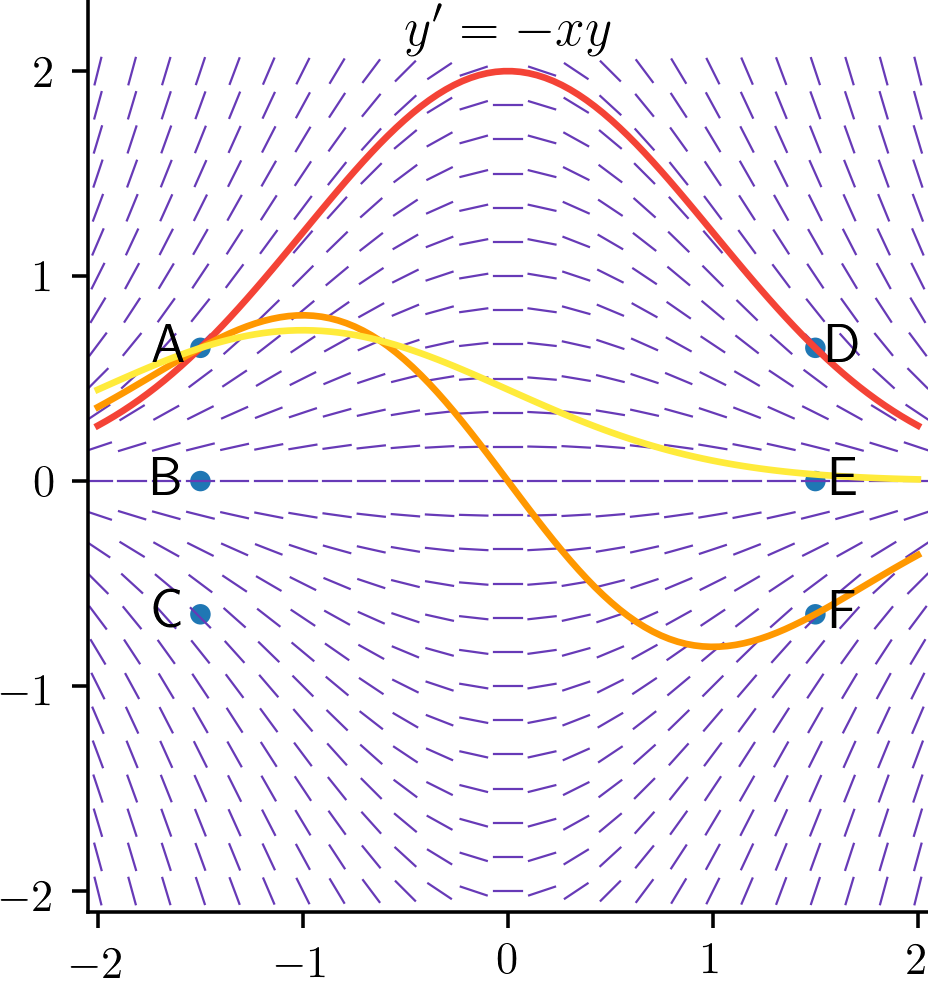
\includegraphics[width=4in]{images/slopeX01.png}
\end{image}
\end{center}
\begin{itemize}
\item The first step is to find a first-order ODE that is satisfied by the family. This involves differentiating with respect to $x$. We get
\[ 4 x^3 + 2y y' = 0, \ \text{ meaning } y' = \answer{-\frac{2x^3}{y}}. \]
\item If $m$ and $m'$ are slopes of orthogonal lines, then $m m' = -1$. So the orthogonal trajectories satisfy an ODE similar to the one above except that the formula for $y'$ is replaced by its negative reciprocal, i.e.,
\[ y' = \answer{\frac{y}{2x^3}}. \]
\item This is a separable ODE. It separates to
\[ \frac{dy}{\answer{y}} = \frac{1}{2} \frac{dx}{\answer{x^3}}. \]
Integrating both sides gives
\[ \ln |y| = - \frac{1}{4} x^{-2} + C. \]
If we exponentiate both sides and reexpress the arbitrary constant, we get
\[ y = C \answer{e^{-\frac{1}{4x^2}}} \]
\end{itemize}


\begin{example}
For the family of curves in the plane given by 
\[ y = \frac{1}{C + x^2} \]
(shown in purple)
find a formula for the orthogonal trajectories (shown in red).
\begin{center}
\begin{image}
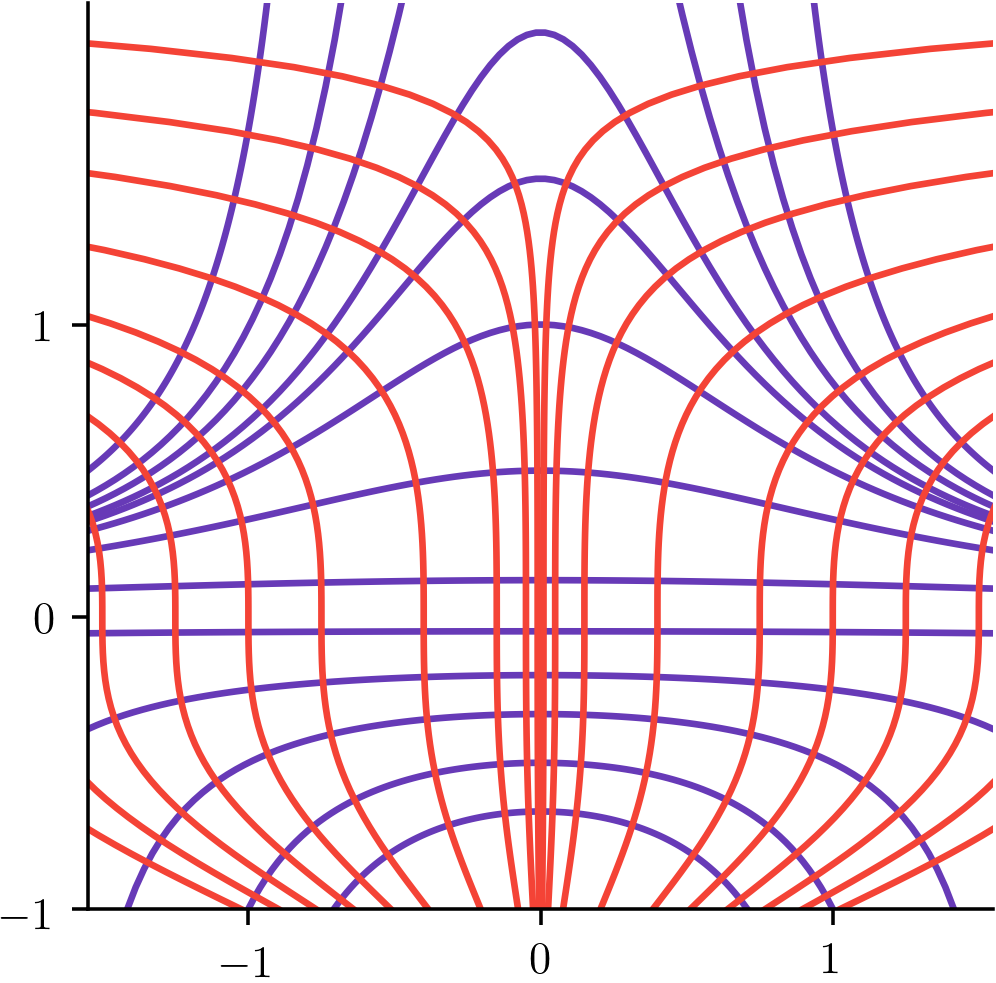
\includegraphics[width=4in]{images/slopeX02.png}
\end{image}
\end{center}
\begin{itemize}
\item We first differentiate with respect to $x$:
\[ y' = \answer{ - \frac{2x}{(x^2+C)^2}}. \]
\item Next we must eliminate $C$ from the equation for $y'$ by using the formula $y = 1/ (x^2+C)$. (For example, solve for $C$ in terms of $x$ and $y$ and then substitute this in to your expression for $y'$.)
\[ y' = \answer{ - 2 x y^2} \]
(your answer here will depend on the variables $x$ and $y$ but should not explicitly depend on $C$).
\item Then we write a new ODE whose slope is the negative reciprocal of the expression we just found:
\[ y' = \answer{\frac{1}{2xy^2}}. \]
This is a separable ODE:
\[ \answer{y^2} dy = \frac{1}{2} \frac{dx}{\answer{x}}. \]
\item Integrate both sides:
\[ \answer{\frac{y^3}{3}} = \frac{1}{2} \answer{\ln |x|} + C. \]
(Don't forget absolute values on logarithms.)
\end{itemize}
\end{example}

\begin{example}

\end{example}


\end{document}
